% =====================================================================
% RESULTS AND DISCUSSION
% Numbers from ../Code/results/part_b.txt ... part_e.txt.
% LLM declaration: text level 3; see the appendix "Use of AI/LLM tools".
% =====================================================================

\section*{Results and discussion}

\subsection*{Part b: sigmoid networks against OLS}

\emph{Design choices.} The input to the network is only $x$, a single standardised column. It does not have to be a polynomial, since the hidden layer makes its own features: node $j$ computes $f(a_jx + c_j)$, with $a_j$ and $c_j$ set by the training, and the output node adds these up with its own weights and bias. Figure~\ref{fig:hinges} shows this for ten ReLU nodes. The output of the network is then
$$
\tilde{y}(x) = b + \sum_{j} w_j \max(0,\, a_j x + c_j),
$$
a sum of hinges with kinks at $x = -c_j/a_j$. The hidden bias $c_j$ moves the kink along $x$, the output bias $b$ moves the curve up and down, and the sum is a piecewise linear curve. With the sigmoid each node is a smooth step instead. One of the ten nodes is inactive on the whole interval, a dead node. The output layer is linear, since $y$ is a real number and a linear output with the MSE is a matched pair.

\begin{figure*}
    \centering
    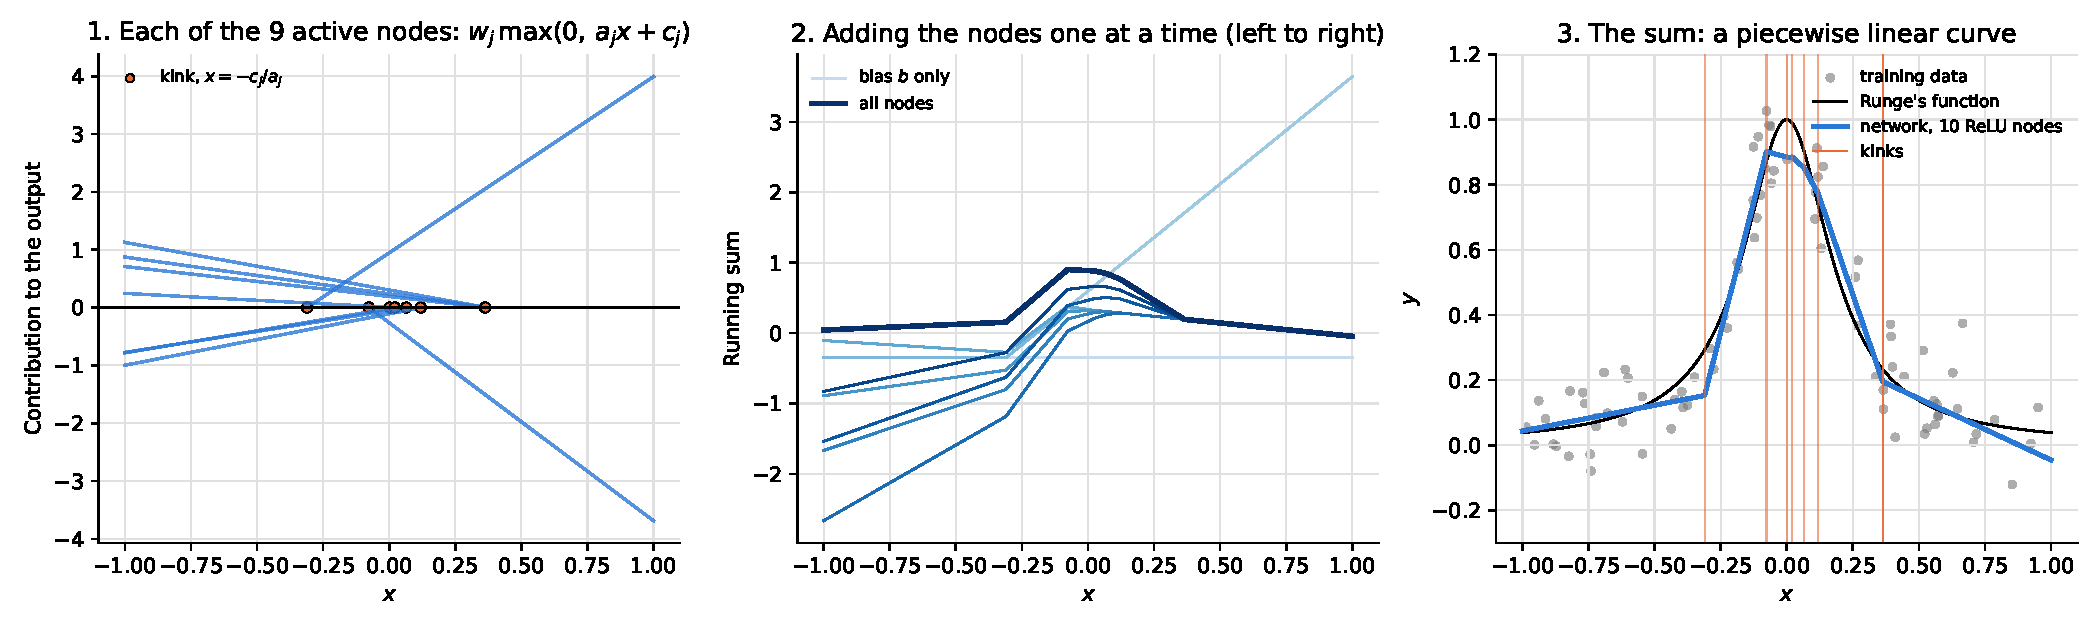
\includegraphics[width=\textwidth]{illustration_relu_hinges.pdf}
    \caption{How a network with one hidden layer of ten ReLU nodes builds its output, trained on the 80 training points of seed 42 (Adam, $\gamma = 3\times10^{-3}$, 4000 epochs). (1) The contribution $w_j\max(0, a_jx + c_j)$ of each node, with its kink at $x = -c_j/a_j$; one node is inactive on the whole interval and not shown. (2) The output bias, and the nodes added one at a time in the order of their kinks. (3) The sum, which is the output of the network, with the kinks marked.}
    \label{fig:hinges}
\end{figure*}

\emph{Learning rates.} Figure~\ref{fig:b_lr} shows the validation MSE after 1000 epochs for one hidden layer of 50 sigmoid nodes. SGD with RMSprop or Adam is best at $\gamma = 10^{-3}$ (0.0065 and 0.0062), below OLS of degree 12 (0.0112) on the same 16 points. Plain GD needs $\gamma = 0.1$ to get down to 0.0137, and blows up at $\gamma = 1$. For smaller $\gamma$ it stays at 0.08--0.10, about the variance of the validation targets (0.079), which is the error of the best constant prediction: the training has hardly started. The factor of 100 between the best learning rates comes from the division by $\sqrt{s}$. RMSprop and Adam take steps of about $\gamma$ for every weight, while GD takes $\gamma$ times the gradient, and the gradients here are small. For large $\gamma$ RMSprop and Adam get worse again, since steps of size $\gamma$ become too coarse. Adam is the least sensitive to $\gamma$, as in Project 1.

\begin{figure}
    \centering
    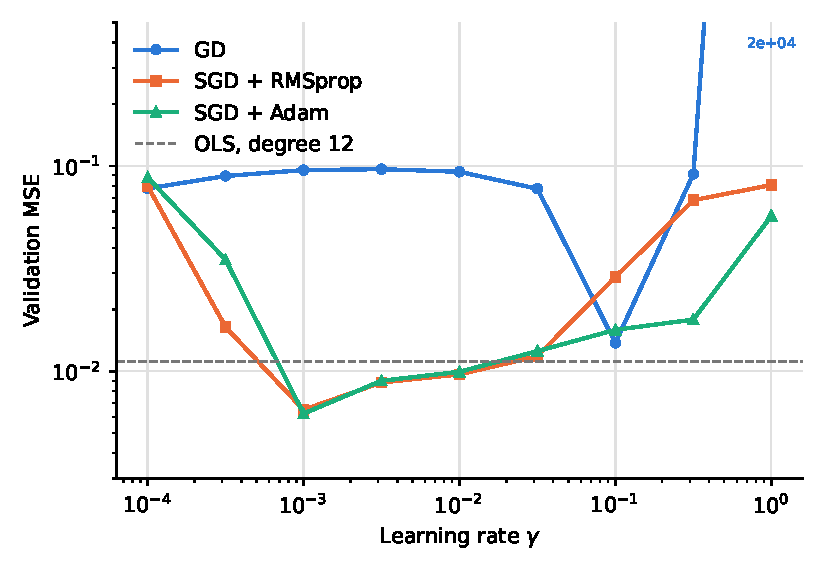
\includegraphics[width=\linewidth]{b_learning_rates.pdf}
    \caption{Validation MSE after 1000 epochs against the learning rate, one hidden layer of 50 sigmoid nodes, trained on 64 points of the seed-42 data set and validated on 16. GD uses all 64 points in each step, SGD minibatches of 16. The number at the top right is the MSE of GD at $\gamma = 1$. Dashed line: OLS of degree 12 fitted to the same 64 points.}
    \label{fig:b_lr}
\end{figure}

\emph{Training curves.} In Fig.~\ref{fig:b_curves} the MSE of GD with $\gamma = 0.1$ first grows to about 200 in six epochs and then falls back. The steps are too long for the curvature of the cost at the start, and in this run the weights moved after a few epochs to where the same step is stable. All three methods then stay on a plateau at about 0.1 for a long time before the MSE falls towards the noise level $\sigma^2 = 0.01$. After 1000 epochs the training MSE is 0.013--0.014 for the SGD methods and 0.030 for GD.

\begin{figure}
    \centering
    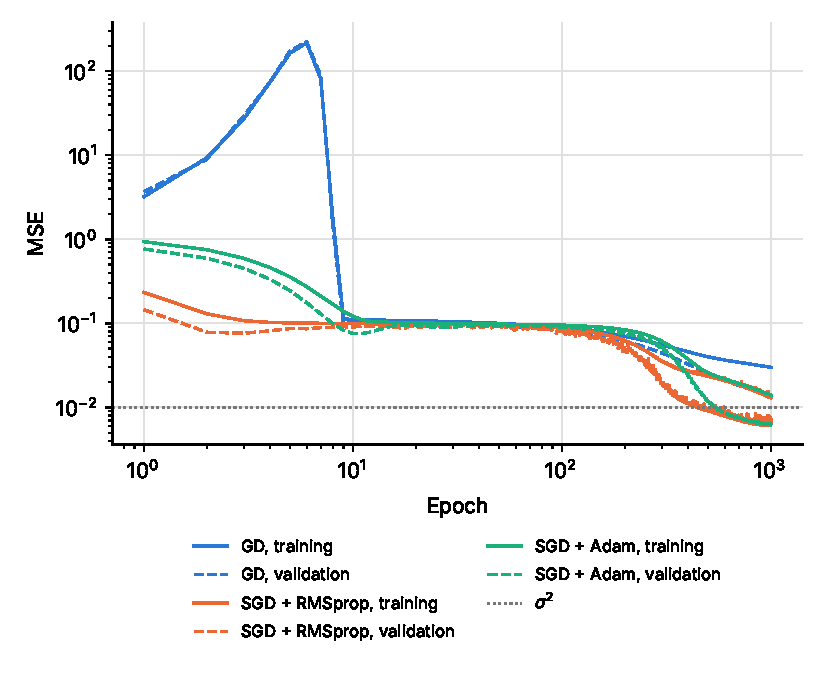
\includegraphics[width=\linewidth]{b_training_curves.pdf}
    \caption{Training (solid) and validation (dashed) MSE after each epoch for the three methods at their best learning rates (GD: $\gamma = 0.1$, RMSprop and Adam: $\gamma = 10^{-3}$), one hidden layer of 50 sigmoid nodes, seed 42. Dotted line: $\sigma^2$.}
    \label{fig:b_curves}
\end{figure}

The validation MSE ends lower than the training MSE, 0.0065 against 0.013 for RMSprop. This is chance in a small validation set: only 3 of the 16 validation points lie near the peak ($|x| < 0.2$), where the fit is hardest, against 18 of the 64 training points, and their noise happens to be smaller (mean squared noise 0.0090 against 0.0103).

\emph{More epochs.} GD is slower, not worse: after 3000 epochs it reaches 0.0068, where RMSprop and Adam were after 1000. Trained longer, RMSprop and Adam get worse (0.0097 and 0.0089 after 3000 epochs), and so does GD after $10\,000$ epochs (0.0101), as the network starts to follow the noise. The number of epochs thus works as a regularisation, like early stopping \cite[Sec.~8.12]{HjorthJensen2026}. The same number of epochs means the same cost, one pass through the data per epoch, but not the same number of updates: SGD makes four per epoch, GD one.

\emph{Architectures.} Table~\ref{tab:b_test} gives the test MSE on the seed-42 split for one and two hidden layers of 50 and 100 nodes, trained on all 80 training points. Only Adam beats OLS (0.0086), with 100 nodes or two layers, and only by a little. GD is clearly worse for all four architectures, but its learning rate was chosen for 50 nodes. None of the 20 test points lie near the peak, so the table mostly measures the flanks.

\begin{table}
    \centering
    \caption{Test MSE on the seed-42 split (20 test points), trained on all 80 training points for 1000 epochs, each method at the learning rate chosen in Fig.~\ref{fig:b_lr}. OLS of degree 12 on the same split: 0.0086.}
    \label{tab:b_test}
    \begin{tabular}{lcccc}
        \toprule
        Hidden layers & Parameters & GD & RMSprop & Adam \\
        \midrule
        50       & 151   & 0.0236 & 0.0123 & 0.0101 \\
        100      & 301   & 0.0651 & 0.0154 & 0.0083 \\
        50, 50   & 2701  & 0.0540 & 0.0111 & 0.0074 \\
        100, 100 & 10401 & 0.0572 & 0.0104 & 0.0078 \\
        \bottomrule
    \end{tabular}
\end{table}

In Fig.~\ref{fig:b_fits} the networks are smoother than the polynomial and do not reach the top of the peak. The polynomial wiggles along the flanks and shoots up above 1 beyond the last training point, at $x = 0.951$. Outside the data a polynomial of high degree cannot be trusted.

\begin{figure}
    \centering
    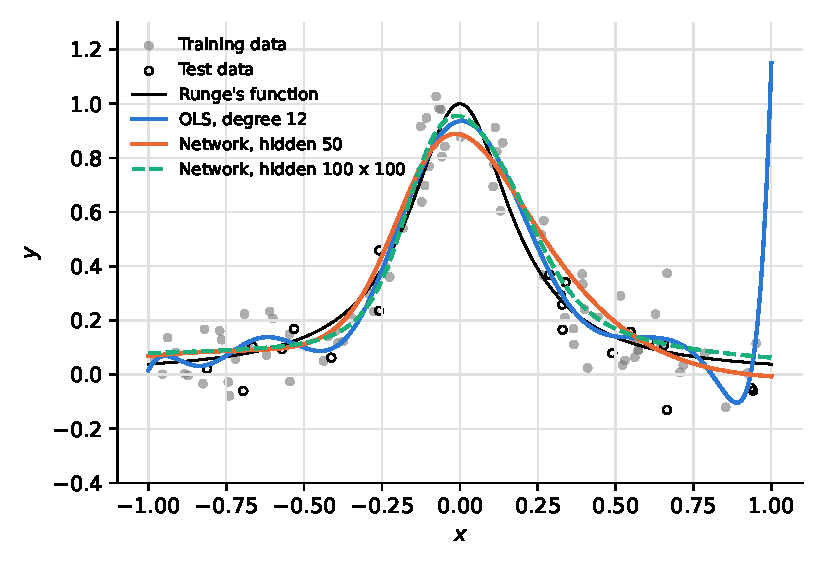
\includegraphics[width=\linewidth]{b_fits.pdf}
    \caption{The seed-42 data, Runge's function, OLS of degree 12 and two sigmoid networks trained with SGD and RMSprop on all 80 training points: one hidden layer of 50 nodes, and two hidden layers of 100 nodes.}
    \label{fig:b_fits}
\end{figure}

\emph{Several data sets.} Over ten data sets (seeds 42--51), with 50 nodes and RMSprop, the median test MSE was 0.0122 for OLS (25th--75th percentile 0.0095--0.0140) and 0.0132 for the network (0.0121--0.0160), and the network was better in only one of the ten. Here OLS of degree 12 is at least as good as the network, and it is a closed-form solution, while the network needs a learning rate, a number of epochs and a random initialisation.

\subsection*{Part c: activation functions, depth and width}

Figure~\ref{fig:c_heat} shows the median validation MSE for 1--5 hidden layers of 5--100 nodes, trained with Adam, $\gamma = 10^{-3}$. The best cells are 0.0125 for the sigmoid (five layers of 10 nodes), 0.0124 for ReLU (two of 10) and 0.0120 for Leaky ReLU (three of 5), and OLS gives 0.0119. Each validation MSE has a standard error of 20--30\,\% (Methods), so most of the differences between the cells are not significant. The sigmoid needs depth: with one hidden layer it stays at 0.017--0.023, and its worst cell, five layers of five nodes (0.068), has a median training MSE of 0.072, so it has hardly started to fit. For ReLU and Leaky ReLU the error is highest with five layers.

\begin{figure*}
    \centering
    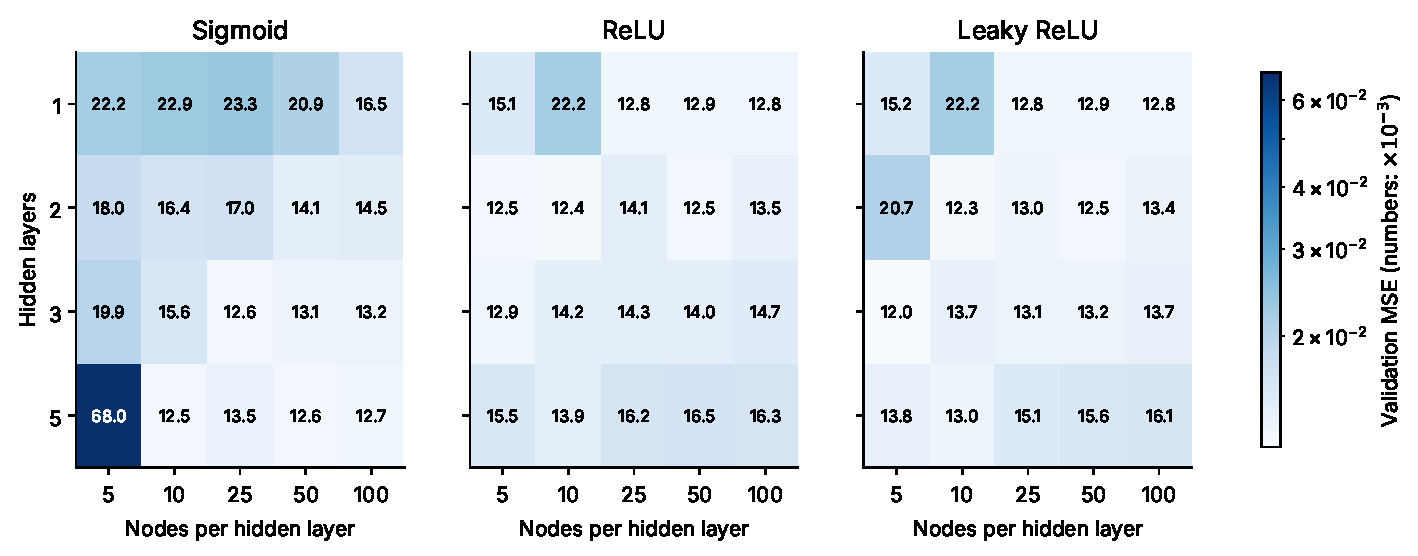
\includegraphics[width=0.9\textwidth]{c_heatmaps.pdf}
    \caption{Median validation MSE over three data sets (seeds 42--44) against the number of hidden layers and of nodes per layer, for sigmoid, ReLU and Leaky ReLU hidden layers; SGD with Adam, $\gamma = 10^{-3}$, minibatches of 16, 1000 epochs. The numbers are the MSE in units of $10^{-3}$, and lighter is better. OLS of degree 12 gives 11.9 on the same validation sets.}
    \label{fig:c_heat}
\end{figure*}

\emph{Overfitting.} In Fig.~\ref{fig:c_over}, with 50 nodes per layer, the training MSE of ReLU and Leaky ReLU falls below $\sigma^2$ as layers are added (about 0.0074 with three and five layers), while the validation MSE grows from 0.0125 with two layers to 0.0165 and 0.0156 with five. With up to $10\,351$ parameters for 64 training points, the networks follow the noise. This is overfitting, as for a high polynomial degree in Project 1. For the sigmoid both curves keep falling, since it learns more slowly. Trained for 5000 epochs instead of 1000, the sigmoid network with five layers reaches a training MSE of 0.0078 and a validation MSE of 0.0144 (0.0085 and 0.0126 after 1000), so it overfits too, only later.

\begin{figure}
    \centering
    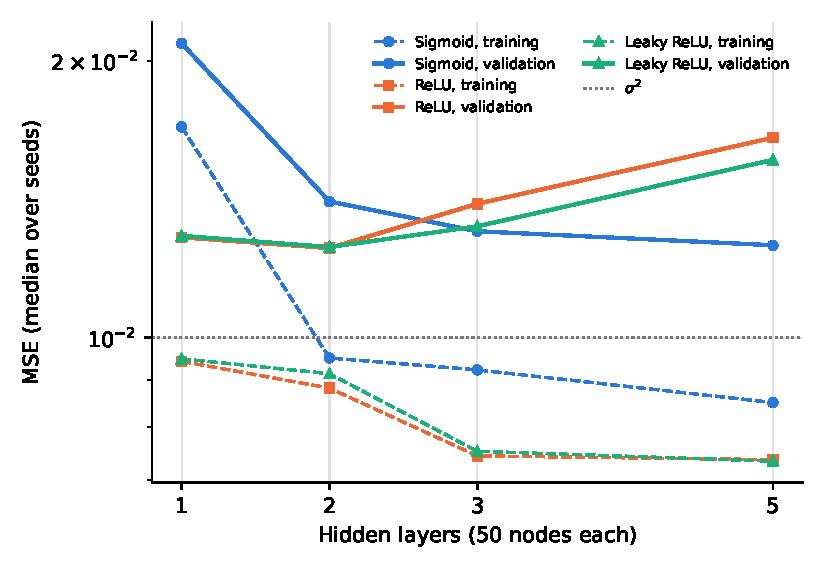
\includegraphics[width=\linewidth]{c_overfitting.pdf}
    \caption{Training (dashed) and validation (solid) MSE against the number of hidden layers of 50 nodes, median over seeds 42--44, from the same runs as Fig.~\ref{fig:c_heat}. Dotted line: $\sigma^2$.}
    \label{fig:c_over}
\end{figure}

\emph{Vanishing gradients.} Figure~\ref{fig:c_grad} shows the root mean square of the weight gradient in each layer of a network with five hidden layers of 50 nodes. For the sigmoid at initialisation it falls from 0.79 in the output layer to $10^{-5}$ in the first hidden layer, by a factor of about 4--5 per layer in the middle of the network. Each layer on the way back multiplies $\boldsymbol{\delta}$ by the transposed weights and by $\sigma'(z) \le 1/4$, so the gradient shrinks geometrically towards the input \cite[Sec.~8.9]{HjorthJensen2026}. With ReLU, whose derivative is 1 for active nodes, and He initialisation, it is 0.1--0.2 in all hidden layers. After 100 epochs the sigmoid gradients in the hidden layers are still about 6 to 50 times smaller than the ReLU gradients, which fits with the sigmoid needing more epochs. We used the root mean square per weight, and not the norm of the whole matrix as in Fig.~8.14 of the lecture notes, because the first and the last layer have 50 weights and the others 2500, and the norm grows with the number of weights.

\begin{figure*}
    \centering
    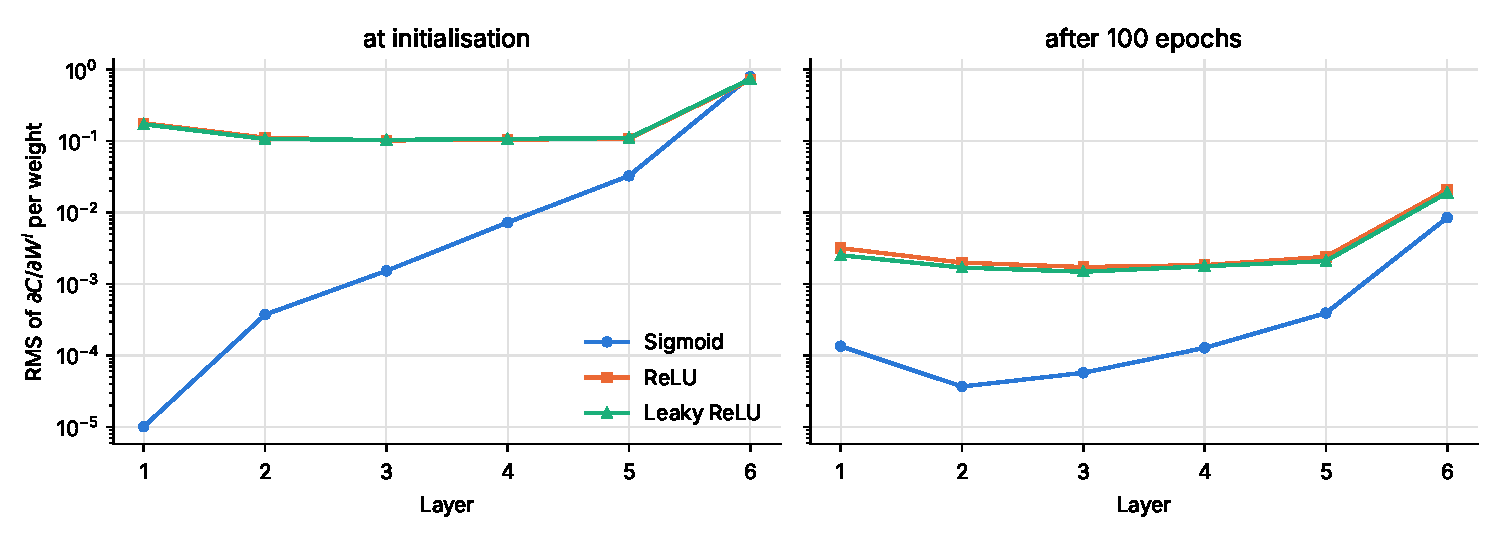
\includegraphics[width=0.85\textwidth]{c_gradient_norms.pdf}
    \caption{Root mean square of $\partial C/\partial \mathbf{W}^l$ over the weights of each layer, for a network with five hidden layers of 50 nodes (layer 1: first hidden layer, layer 6: output layer), on the 64 training points of seed 42. Left: at initialisation. Right: after 100 epochs with Adam, $\gamma = 10^{-3}$.}
    \label{fig:c_grad}
\end{figure*}

\emph{Which activation?} For this problem the three activations reach the same level in their best configurations. The sigmoid needs more layers or more epochs, because its gradients vanish towards the input. ReLU and Leaky ReLU learn faster, but overfit when the network gets deep. Leaky ReLU, which cannot have completely dead nodes, gave practically the same results as ReLU.

\subsection*{Part d: $L_1$ and $L_2$ penalties}

For the penalties we used the ReLU network with three hidden layers of 50 nodes, which overfits in part c. In Fig.~\ref{fig:d_heat} the best cell for $L_2$ has $\lambda = 0$ (0.0123), and the best for $L_1$ has $\lambda = 10^{-6}$ (0.0120), which is no real difference. $\lambda = 10^{-2}$ is clearly worse (0.015--0.027): it pulls the weights so hard that the network can no longer follow the function, as a large $\lambda$ did in Ridge and Lasso. Both grids are best at the smallest learning rate, $\gamma = 10^{-4}$, at the edge of the grid. With this $\gamma$ the network does not get far enough in 1000 epochs to follow the noise, so the learning rate and the fixed number of epochs already regularise the network, and the penalty has little left to do. At larger $\gamma$ moderate penalties do somewhat better than $\lambda = 0$, for instance 0.0127 against 0.0140 for $L_2$ with $\lambda = 10^{-4}$ at $\gamma = 10^{-3}$, but within the uncertainty.

\begin{figure*}
    \centering
    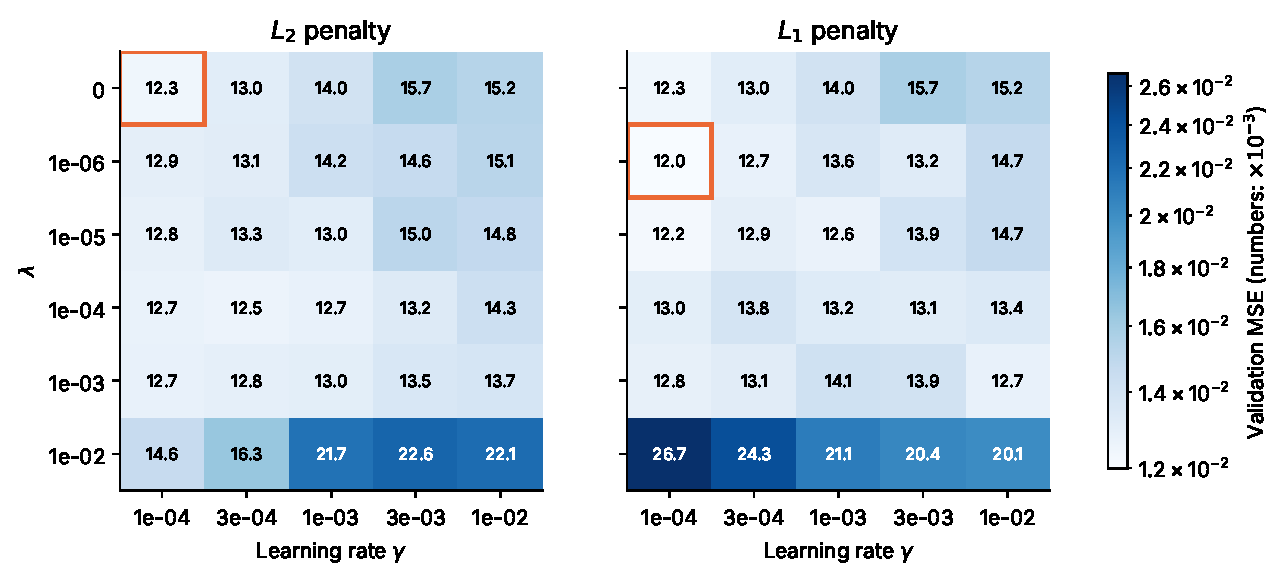
\includegraphics[width=0.8\textwidth]{d_heatmaps.pdf}
    \caption{Median validation MSE over seeds 42--44 against the learning rate $\gamma$ and the penalty $\lambda$, for the $L_2$ (left) and $L_1$ (right) penalty; three hidden layers of 50 ReLU nodes, Adam, minibatches of 16, 1000 epochs. The numbers are the MSE in units of $10^{-3}$, and the orange square marks the lowest value. The row $\lambda = 0$ is the same in both panels.}
    \label{fig:d_heat}
\end{figure*}

Table~\ref{tab:d_test} gives the test MSE on the 20 data sets of Project 1. Since $\lambda = 0$ was best for $L_2$, the $L_2$ network is the network without penalty. Its median, 0.0093, is lower than for Ridge (0.0133), Lasso (0.0139) and OLS (0.0155), and close to the median mean squared noise of 0.0091, which is what even the true function gets. Its 75th percentile (0.0116) is below the median of Ridge. The hyperparameters were chosen on the validation sets of seeds 42--44, so the test sets played no part in the choice.

\begin{table}
    \centering
    \caption{Test MSE on the 20 data sets of Project 1 (seeds 42--61): median and 25th--75th percentile over the data sets. Networks: three hidden layers of 50 ReLU nodes, Adam, $\gamma = 10^{-4}$, 1000 epochs on all 80 training points. Project 1: degree and $\lambda$ chosen by 5-fold cross-validation. Noise: the mean squared noise $(y_i - f(x_i))^2$ in the test sets.}
    \label{tab:d_test}
    \begin{tabular}{lcc}
        \toprule
        Model & Median & Percentiles \\
        \midrule
        Network, no penalty                 & 0.0093 & 0.0084--0.0116 \\
        Network, $L_1$, $\lambda = 10^{-6}$ & 0.0096 & 0.0083--0.0119 \\
        OLS (Project 1)                     & 0.0155 & -- \\
        Ridge (Project 1)                   & 0.0133 & -- \\
        Lasso (Project 1)                   & 0.0139 & -- \\
        Noise                               & 0.0091 & -- \\
        \bottomrule
    \end{tabular}
\end{table}

So the penalty is not why the network beats Ridge and Lasso. In Project 1 the largest errors of the polynomials came from data sets where they had to extrapolate or bridge a gap near the edges of the interval. The ReLU network continues as a straight line outside its outermost kinks and cannot oscillate like a polynomial of high degree, so it avoids these errors. In Project 1, Ridge improved on OLS by keeping the high-degree polynomials from blowing up; for the network, the small learning rate already prevents overfitting. The Lasso solver of Project 1 did not converge for the small $\lambda$ chosen by cross-validation, so the Lasso numbers are approximate. The network also differs from the one in part b in the activation, the depth, the optimiser and the learning rate, and we did not test which of these made it better than OLS.

\subsection*{Part e: classification of MNIST}

All the MNIST networks have 784 inputs, a softmax output layer of 10 nodes and the cross entropy as cost, and were trained with Adam in minibatches of 128 for 20 epochs, with the $L_2$ penalty.

\emph{Learning rate and penalty.} In Fig.~\ref{fig:e_heat}, for one hidden layer of 100 ReLU nodes, the best combination is $\gamma = 10^{-3}$ and $\lambda = 10^{-5}$ (0.9783), but for $\lambda \le 10^{-4}$ the differences are within the standard error of 0.0014. $\lambda = 10^{-3}$ is too strong (0.9640 at $\gamma = 10^{-3}$), $\gamma = 10^{-4}$ is too slow for 20 epochs (about 0.95), and $\gamma = 3\times10^{-3}$ is a little worse than $10^{-3}$. As for the Runge data, the penalty gave no measurable gain. The validation accuracy (Fig.~\ref{fig:e_curves}) flattens out at about 0.98 after ten epochs without a downward trend, so there is no clear overfitting for the penalty to remove.

\begin{figure}
    \centering
    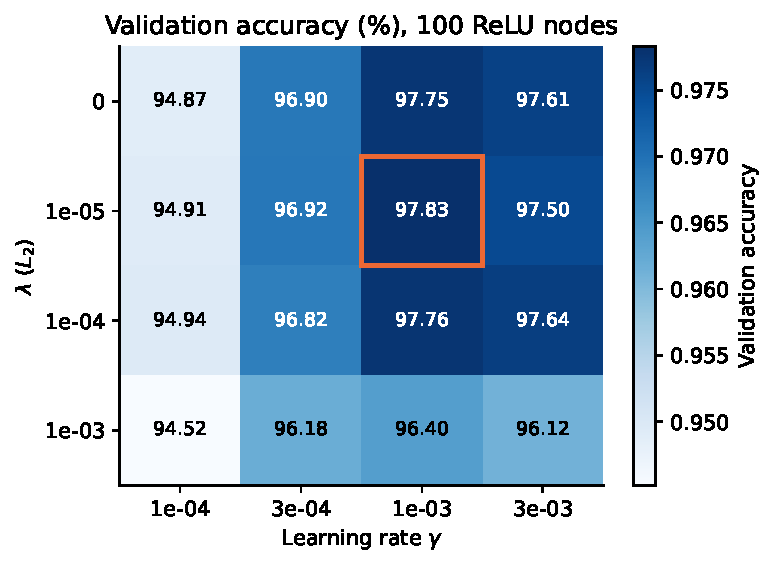
\includegraphics[width=0.9\linewidth]{e_heatmap.pdf}
    \caption{Validation accuracy in percent on MNIST against the learning rate $\gamma$ and the $L_2$ penalty $\lambda$; one hidden layer of 100 ReLU nodes, Adam, minibatches of 128, 20 epochs. The orange square marks the best value. The standard error of each number is about 0.14 percentage points.}
    \label{fig:e_heat}
\end{figure}

\begin{figure}
    \centering
    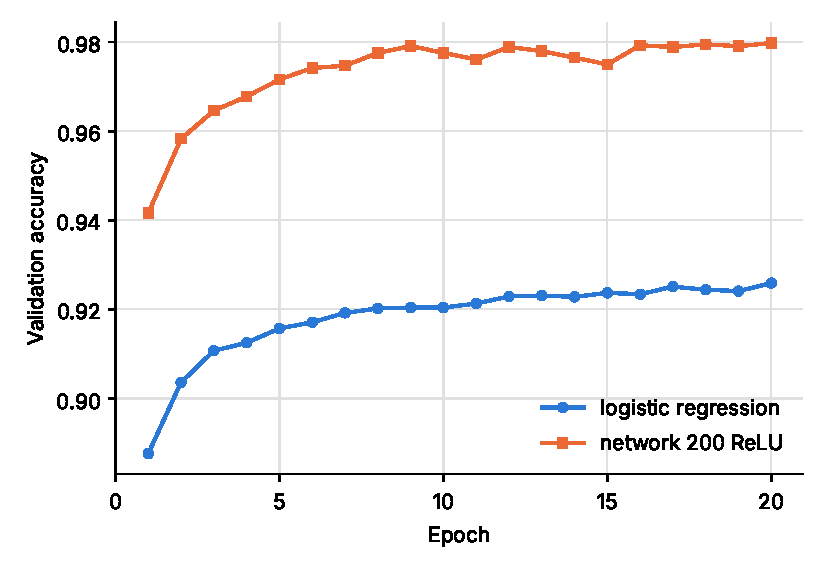
\includegraphics[width=\linewidth]{e_training_curves.pdf}
    \caption{Validation accuracy after each epoch for logistic regression ($\gamma = 10^{-3}$) and for the network with one hidden layer of 200 ReLU nodes ($\gamma = 10^{-3}$, $\lambda = 10^{-5}$).}
    \label{fig:e_curves}
\end{figure}

\emph{Architecture and activation.} In Table~\ref{tab:e_arch}, wider is better up to 200 nodes, and two layers of 100 nodes are not better than one layer of 200. ReLU and Leaky ReLU are equal, and the sigmoid is 0.2--0.5 percentage points lower. We chose one hidden layer of 200 ReLU nodes (0.9798), but Leaky ReLU with 200 nodes (0.9795) is within the standard error. A single run also depends on chance in the training. With other seeds for the initial weights and the minibatch order, the same network reached 0.9798, 0.9795 and 0.9703 after 20 epochs. The low value is a dip in the last epoch; one epoch earlier that run was at 0.9795. With a constant learning rate Adam does not settle at a minimum, and over the last ten epochs each of the three runs varied by 0.35 to 0.92 percentage points. Differences of a few tenths of a percentage point between the cells are therefore not meaningful.

\begin{table}
    \centering
    \caption{Validation accuracy on MNIST for different hidden layers and activations, at $\gamma = 10^{-3}$ and $\lambda = 10^{-5}$, after 20 epochs. The standard error is about 0.0014.}
    \label{tab:e_arch}
    \begin{tabular}{lcccc}
        \toprule
        Activation & 50 & 100 & 200 & 100, 100 \\
        \midrule
        Sigmoid    & 0.9633 & 0.9730 & 0.9762 & 0.9753 \\
        ReLU       & 0.9669 & 0.9783 & 0.9798 & 0.9773 \\
        Leaky ReLU & 0.9684 & 0.9783 & 0.9795 & 0.9769 \\
        \bottomrule
    \end{tabular}
\end{table}

\emph{Test results.} The test set was used once, for the chosen network, for logistic regression at its best learning rate ($\gamma = 10^{-3}$) and for the scikit-learn models:

\noindent\begin{minipage}{\linewidth}
\begin{lstlisting}[style=terminal]
Test set (10000 images), used once
  most frequent digit              accuracy 0.1135
  logistic regression              accuracy 0.9273 +- 0.0026
  network 200 ReLU                 accuracy 0.9777 +- 0.0015
  scikit-learn LogisticRegression  accuracy 0.9245
  scikit-learn MLPClassifier       accuracy 0.9797
\end{lstlisting}
\end{minipage}

The network makes 223 errors on the $10\,000$ test images, against 727 for logistic regression, 69\,\% fewer. scikit-learn gets nearly the same accuracies with the same models, which supports our implementation; its network also differs from ours in the initialisation and the penalty. Logistic regression on raw pixels is known to give about 92\,\%, and convolutional networks above 99\,\% \cite{LeCun1998}. The network took about eight times longer to train than logistic regression (74\,s against 9\,s on our machine).

\emph{Why the hidden layer helps.} Logistic regression computes one score per digit, a weighted sum over the pixels $p$,
$$
z_k = \sum_{p} w_{pk}\,x_p + b_k ,
$$
so the weights of digit $k$ form a $28\times28$ template (top row of Fig.~\ref{fig:weights}). The score is high when the image has ink where the template is positive (red) and none where it is negative (blue). The templates are blurred, since each of them must match every way of writing its digit. The hidden nodes (lower rows) do not belong to any digit. They respond to parts of digits, such as strokes in certain places, and the output layer combines them. More weights alone would not help: with a linear activation in the hidden layer, the network would still be a linear function of the pixels. It is the non-linear activation that lets the network combine features, for instance to recognise different ways of writing the same digit, which one linear template per digit cannot.

\begin{figure*}
    \centering
    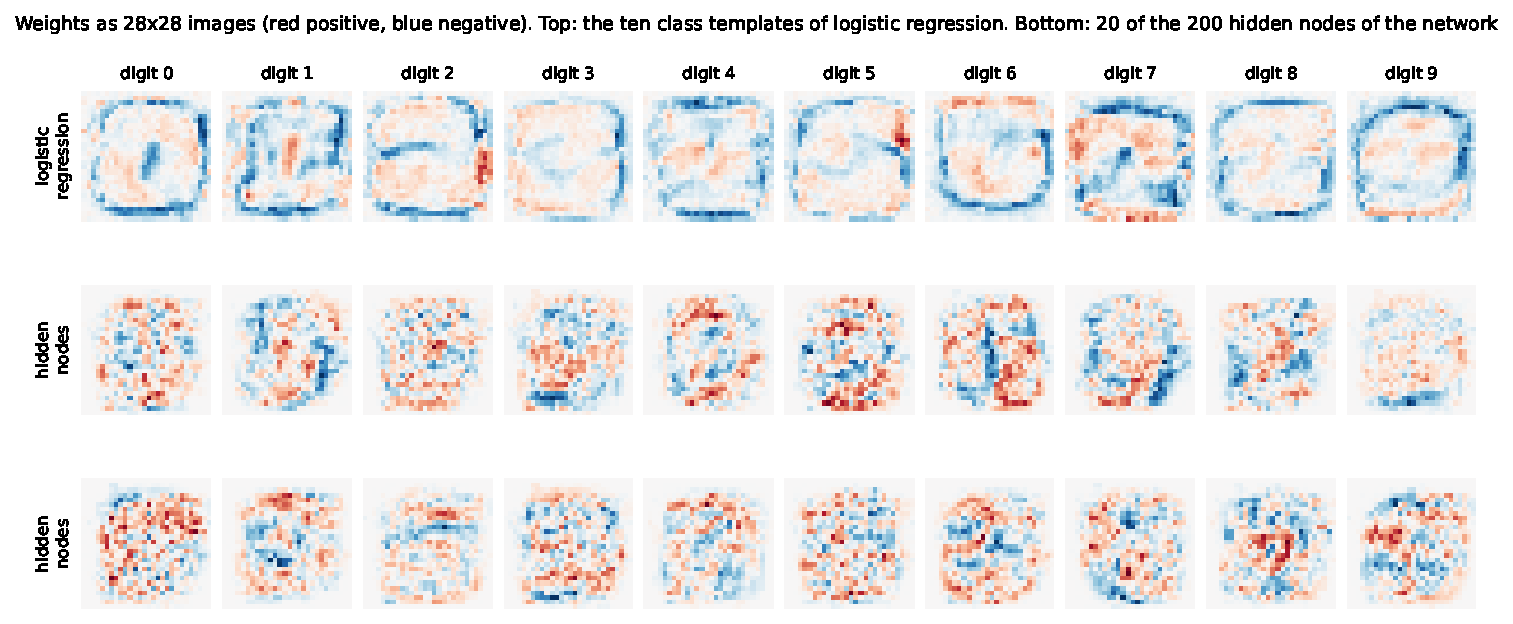
\includegraphics[width=0.85\textwidth]{illustration_mnist_weights.pdf}
    \caption{The weights from the 784 pixels shown as $28\times28$ images (red positive, blue negative, each image on its own colour scale). Top row: the ten digit templates of logistic regression. Lower rows: the weights into 20 of the 200 hidden nodes of the network, chosen at random.}
    \label{fig:weights}
\end{figure*}

\emph{Which errors remain?} The errors in Fig.~\ref{fig:e_conf} are concentrated in pairs of digits that can look alike: 2 classified as 8 (14 images), 4 as 9 (14), 9 as 7 (8), 2 as 7 (8), and 5 as 6 and as 3 (7 each). The precision is lowest for 8 (0.954), so other digits are often classified as 8, and the recall is lowest for 2 (0.961) and 9 (0.967), so these are most often classified as something else. The network reduced the errors most for the digits that logistic regression found hardest: 5 (from 116 to 25), 2 (109 to 40), 9 (100 to 33), 8 (95 to 23) and 3 (81 to 19). The accuracy alone shows none of this.

\begin{figure*}
    \centering
    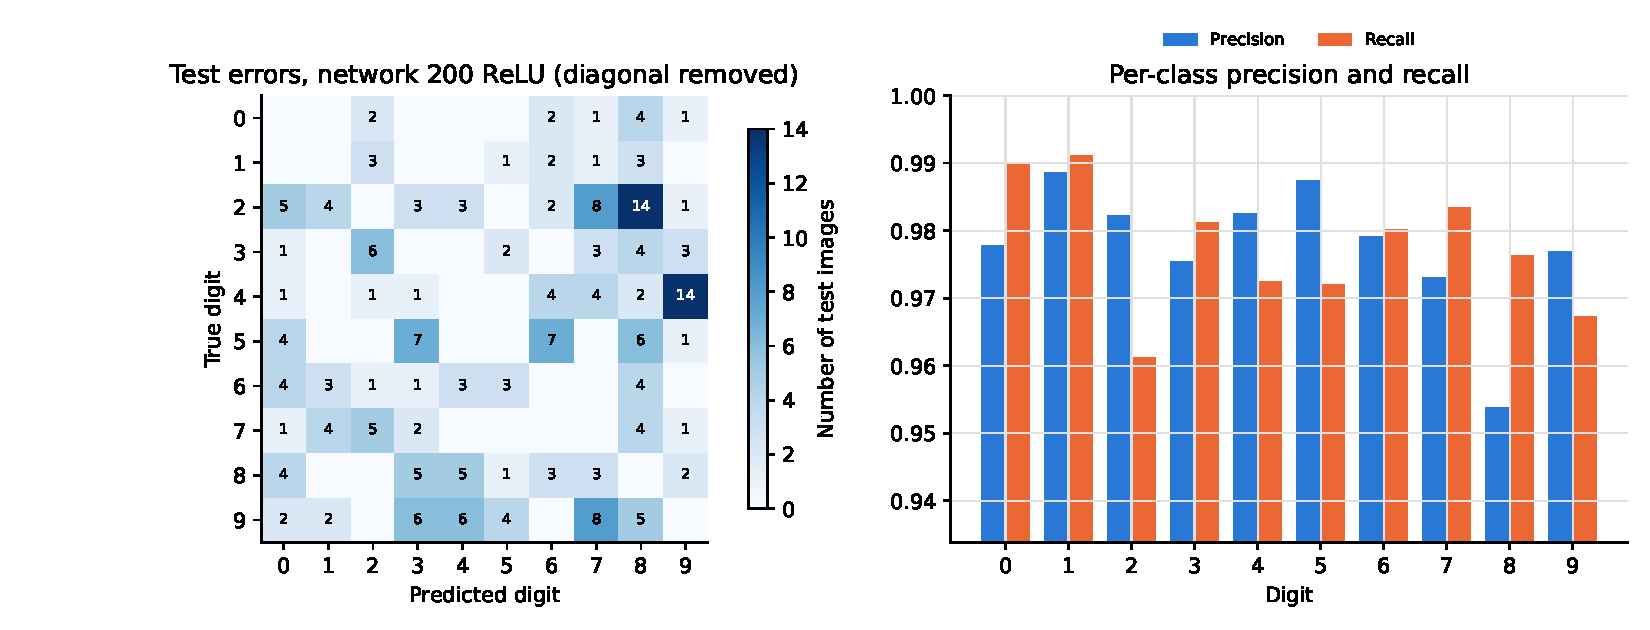
\includegraphics[width=0.85\textwidth]{e_confusion.pdf}
    \caption{Left: the confusion matrix of the network with 200 ReLU nodes on the $10\,000$ test images, with the diagonal (the correct answers) removed so that the errors are visible. Right: precision and recall for each digit.}
    \label{fig:e_conf}
\end{figure*}
